\documentclass[12pt]{article}

\usepackage[brazilian]{babel}
\usepackage[utf8]{inputenc}
\usepackage[T1]{fontenc}
\usepackage{multirow}
\usepackage{lscape}
\usepackage{latexsym}
\usepackage{amscd}
\usepackage{amsfonts}
\usepackage{epsf}
\usepackage{times}
\usepackage{multicol}
\usepackage{subfigure}
\usepackage{graphicx}
\usepackage{gensymb}
\usepackage{caption}
\usepackage{multicol}
\usepackage{tabularx}
\usepackage{amsmath}
\usepackage{indentfirst}

\newcommand{\HRule}{\rule{\linewidth}{0.5mm}}
\renewcommand{\thefootnote}{\fnsymbol{footnote}}

\special{papersize=21.59cm,27.94cm}
\usepackage[top=3cm,left=2cm,right=2cm,bottom=3cm]{geometry}
\linespread{1.45}

% Inicio %%%%%%%%%%%%%%%%%%%%%%%%%%%%%%%%%%%%%%%%%%%%%%%%%%%%%%%%%%%%%%%%%%%%%%

\begin{document}

% Capa %%%%%%%%%%%%%%%%%%%%%%%%%%%%%%%%%%%%%%%%%%%%%%%%%%%%%%%%%%%%%%%%%%%%%%%%

\begin{titlepage}

\begin{center}


% Upper part of the page
\begin{center}
  \begin{figure}[t]
    \centering
    \subfigure{
\includegraphics[width=1.5cm]{unicamp.png}}
    \hfill
    \subfigure{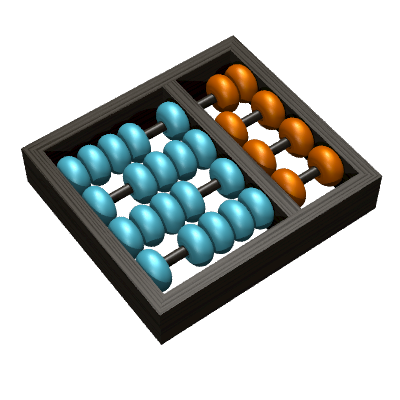
\includegraphics[width=2cm]{ic.png}}
  \end{figure}
\end{center}

\textsc{\LARGE UNICAMP}\\[1.5cm]

\textsc{\Large MC613 - Laboratório de Circuitos Digitais}\\[0.5cm]


% Title
\HRule \\[0.4cm]
{ \huge \bfseries Campo Minado}\\[0.1cm]
\HRule \\[1.5cm]

% Author and supervisor
\begin{minipage}{0.4\textwidth}
\begin{flushleft} \large
\emph{Autores:}\\
Caian \textsc{Benedicto} - 105896\\
Brunno \textsc{Arangues} - 105881\\
\emph{Grupo:} B22\\
\end{flushleft}
\end{minipage}
\begin{minipage}{0.4\textwidth}
\begin{flushright} \large
\emph{Professor:} \\
Guido \textsc{Araújo} \\
\emph{Auxiliar:} \\
Caio \textsc{Hoffman} \\
\end{flushright}
\end{minipage}

\vfill

% Bottom of the page
{\large \today}

\end{center}

\end{titlepage}

% Sobre o jogo %%%%%%%%%%%%%%%%%%%%%%%%%%%%%%%%%%%%%%%%%%%%%%%%%%%%%%%%%%%%%%%%

\section{Sobre o jogo}
\label{sec:gameinfo}

O Campo Minado (\emph{Minesweeper}) é um jogo clássico de Windows onde o
objetivo principal é abrir todos os campos que não são minas. Todo campo ainda
não aberto pode ser marcado com uma bandeira como auxílio visual que esse campo
pode ser uma mina. Ao ser aberto, um campo pode conter: 

\begin{enumerate}

	\item Uma mina, nesse ponto o jogo acaba com uma derrota, revelando as 
		demais minas no jogo.
		
	\item Um espaço vazio, indica que o campo não enxerga nenhuma mina nos
		8 campos que o cerca. Por comodidade esses campos adjacentes também são
		abertos, caso haja outro espaço vazio em um desses campos uma recursão
		ocorre até que todos o espaços vazios vizinhos sejam abertos.
		
	\item Um número, indica quantos dos 8 campos vizinhos são minas, o jogador
		deve utilizar essa informação para evitar as minas e ganhar o jogo.

\end{enumerate}

Além do campo minado a tela também mostra um contador de tempo, que se inicia
na primeira jogada quando o jogador abre um campo e para quando o jogo acaba
(seja por vitória ou derrota), existe também um contador de minas indicando
quantas minas ainda faltam ser encontradas, esse contador decresce quando o
jogador marca um campo com a bandeira, ele não influencia na lógica de
vitória e derrota, apenas serve como um auxílio. Ambos os contadores possuem
um limite superior de $999$ e, especificamente para o contador de minas, um
limite inferior de $0$.

Em particular, a nossa implementação permite selecionar nas \emph{switches}
a quantidade de minas a serem colocadas no jogo ao ser reiniciado. O valor
escolhido é mostrado imediatamente no \emph{display} de 7 segmentos mas só
irá alterar o jogo quando for reiniciado. O jogo pode ser reiniciado com
a \emph{key} 1, um \emph{reset} geral de todos os módulos é feito na
\emph{key} 0.

\begin{figure}[ht!]
	\centering
	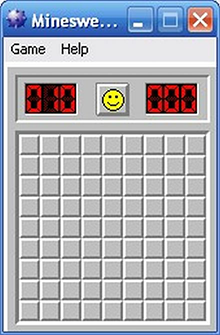
\includegraphics[scale=0.75]{img/game.png}
	\vspace{3mm}
	\caption{Campo minado no Windows XP}
	\label{fig:game}
\end{figure}

% Componentes %%%%%%%%%%%%%%%%%%%%%%%%%%%%%%%%%%%%%%%%%%%%%%%%%%%%%%%%%%%%%%%%%

\section{Componentes do projeto}
\label{sec:components}

% Visao Geral %%%%%%%%%%%%%%%%%%%%%%%%%%%%%%%%%%%%%%%%%%%%%%%%%%%%%%%%%%%%%%%%%

\subsection{Visão geral}
\label{sec:overview}

A figura~\ref{fig:overview} ilustra a conexão e o sentido do fluxo de dados
entre os principais componentes dentro do \emph{top-level} e com módulos
externos. Sinais de \emph{reset} e \emph{clock} não foram explicitados.

\begin{figure}[ht!]
	\centering
	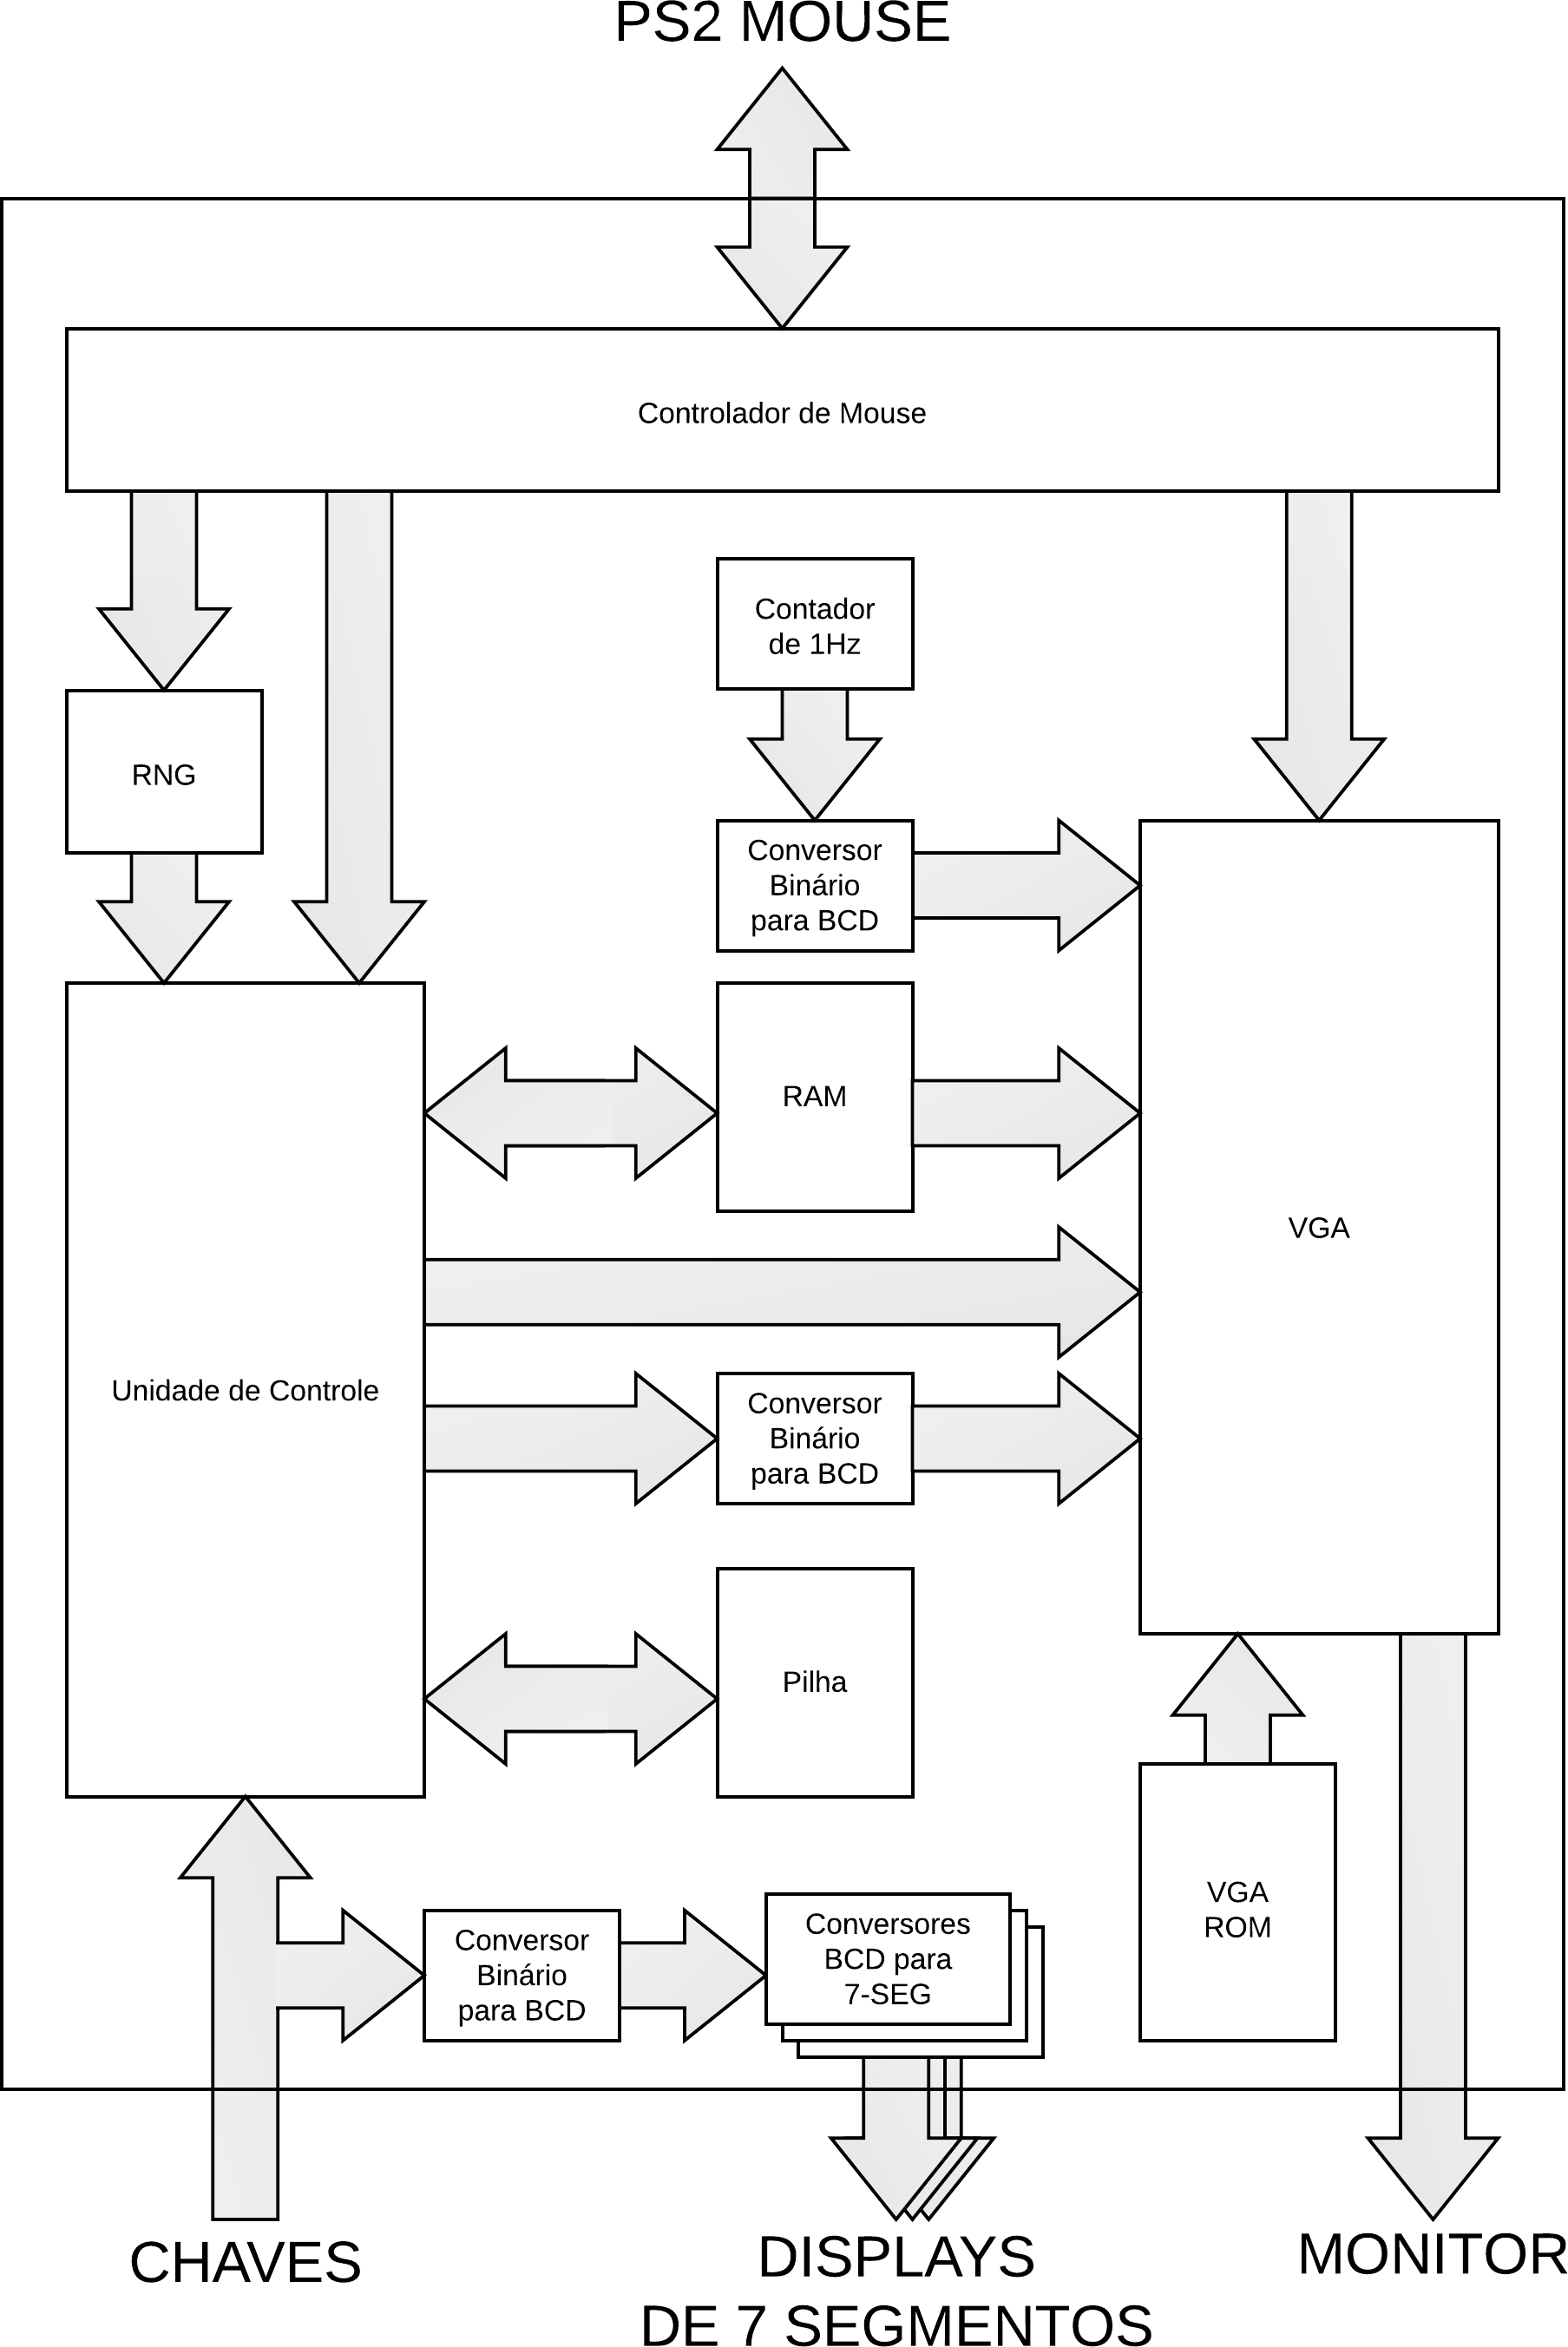
\includegraphics[scale=0.85]{img/overview.png}
	\vspace{3mm}
	\caption{Comunicação entre os componentes no top-level}
	\label{fig:overview}
\end{figure}

% RAM %%%%%%%%%%%%%%%%%%%%%%%%%%%%%%%%%%%%%%%%%%%%%%%%%%%%%%%%%%%%%%%%%%%%%%%%%

\subsection{RAM}
\label{sec:ram}

{\bf Módulo principal:} \verb|ram.vhd|

{\bf Descrição:} A RAM é a memória principal do projeto, ela é instanciada a 
partir de um componente de memória disponível na biblioteca \emph{lpm} do 
Quartus e permite 2 canais de leitura e escrita a \emph{clocks} diferentes. 
Ela é utilizada tanto pela unidade de controle (leitura e escrita) quanto pela
VGA (apenas leitura) e funciona isolando a lógica de jogo da lógica de síntese
da imagem final.

\subsubsection{Endereçamento}
\label{sec:ramaddr}

A memória possui 2048 palavras das quais 1200 são utilizadas para representar
as 30 linhas por 40 colunas de elementos na tela, sejam eles parte integrante
do campo minado ou apenas elementos estruturais, contadores e o rosto amarelo.
O endereçamento dos elementos é feito diretamente com a respectiva linha e 
coluna do elemento: 

\begin{table}[ht!]
\centering
\begin{tabular}{l|c|c|c|c|c|c|c|c|c|c|c|}
\cline{2-12}
Bit: & 10 & 9 & 8 & 7 & 6 & 5 & 4 & 3 & 2 & 1 & 0 \\
\cline{2-12}
 & \multicolumn{5}{c|}{linha} & \multicolumn{6}{c|}{coluna}\\
\cline{2-12}
\end{tabular}
\caption{Endereçamento de elementos na memória}
\label{tab:ramaddr}
\end{table}

\subsubsection{Codificação}
\label{sec:ramenc}

Cada palavra possui 8 bits, organizados de forma a facilitar a lógica tanto
pela unidade de controle quanto pela VGA. Cada elemento salvo na RAM pode
pertencer a uma de 4 classes possíveis, determinadas pelos 2 bits mais
significativos, como indicado na tabela~\ref{tab:rammsb};

\begin{table}[ht!]
\centering
\begin{tabular}{|c|c|c|}
\hline
\multicolumn{2}{|c|}{Bits} & \multirow{2}{*}{Classe} \\
\cline{1-2}
7 & 6 & \\
\hline
0 & 0 & \multicolumn{1}{|l|}{Estrutural} \\
0 & 1 & \multicolumn{1}{|l|}{Elemento de jogo} \\
1 & 0 & \multicolumn{1}{|l|}{Rosto} \\
1 & 1 & \multicolumn{1}{|l|}{Contador de tempo / mina} \\
\hline
\end{tabular}
\caption{Classes de elementos na memória}
\label{tab:rammsb}
\end{table}

Elementos estruturais incluem as bordas do campo minado, o fundo preto e
o fundo cinza da região onde ficam o rosto e os contadores, esses elementos são
usados apenas pelo módulo VGA e codificam diretamente o índice do respectivo 
ladrilho na ROM gráfica.

\begin{table}[ht!]
\centering
\begin{tabular}{l|c|c|c|c|c|c|c|c|}
\cline{2-9}
Bit: & 7 & 6 & 5 & 4 & 3 & 2 & 1 & 0 \\
\cline{2-9}
 & 0 & 0 & \multicolumn{6}{c|}{índice na ROM}\\
\cline{2-9}
\end{tabular}
\caption{Codificação dos elementos estruturais}
\label{tab:structenc}
\end{table}

Elementos numéricos codificam o dígito (centenas, dezenas e unidades) ao
qual estão associados, se fazem parte da metade superior ou inferior do
número (cada número ocupa 2 ladrilhos da tela) e se estão associados a
contadores de tempo ou de minas. A seleção do número é feita em tempo
real pelo módulo de VGA.

\begin{table}[ht!]
\centering
\begin{tabular}{l|c|c|c|c|c|c|c|c|}
\cline{2-9}
Bit: & 7 & 6 & 5 & 4 & 3 & 2 & 1 & 0 \\
\cline{2-9}
 & 1 & 1 & 0 & 0 & S & \multicolumn{3}{c|}{Modo}\\
\cline{2-9}
\end{tabular}

\vspace{5mm}

\begin{tabular}{|c|l|}
\hline
\multirow{2}{*}{S} & 0 - Metade superior do número \\
				   & 1 - Metade inferior do número \\
\hline
\multirow{6}{*}{Modo} & 000 - Unidade de tempo \\
					  & 001 - Dezena de tempo \\
					  & 010 - Centena de tempo \\
					  & 011 - Unidade de minas \\
					  & 100 - Dezena de minas \\
					  & 101 - Centena de minas \\
\hline
\end{tabular}

\caption{Codificação dos elementos numéricos}
\label{tab:numenc}
\end{table}

Elementos de face codificam qual dos 4 quadrantes eles estão associados.
A seleção entre o rosto normal, surpreso, morto e vitorioso também é
feita em tempo real pelo módulo de VGA.

\begin{table}[ht!]
\centering
\begin{tabular}{l|c|c|c|c|c|c|c|c|}
\cline{2-9}
Bit: & 7 & 6 & 5 & 4 & 3 & 2 & 1 & 0 \\
\cline{2-9}
 & 1 & 0 & 0 & 0 & 0 & 0 & S & L \\
\cline{2-9}
\end{tabular}

\vspace{5mm}

\begin{tabular}{|c|l|}
\hline
\multirow{2}{*}{S} & 0 - Metade superior do rosto \\
				   & 1 - Metade inferior do rosto \\
\hline
\multirow{2}{*}{L} & 0 - Metade esquerda do rosto \\
				   & 1 - Metade direita do rosto \\
\hline
\end{tabular}

\caption{Codificação dos elementos de face}
\label{tab:faceenc}
\end{table}

Elementos de jogo possuem a codificação mais elaborada das 4 classes, ela
indica o número de minas que o campo enxerga em seus vizinhos, indica se o
campo foi aberto pelo jogador, se ele foi marcado com uma bandeira e se é uma
mina.

\begin{table}[ht!]
\centering
\begin{tabular}{l|c|c|c|c|c|c|c|c|}
\cline{2-9}
Bit: & 7 & 6 & 5 & 4 & 3 & 2 & 1 & 0 \\
\cline{2-9}
 & 0 & 1 & C & F & \multicolumn{4}{c|}{Modo}\\
\cline{2-9}
\end{tabular}

\vspace{5mm}

\begin{tabular}{|c|l|}
\hline
\multirow{2}{*}{C} & 0 - Campo fechado pelo jogador \\
				   & 1 - Campo aberto pelo jogador \\
\hline				   
\multirow{2}{*}{F} & 0 - Campo não marcado com bandeira \\
				   & 1 - Campo marcado com bandeira \\				   
\hline
\multirow{2}{*}{Modo} & 0000 ... 1000 - Número de minas vistas nos vizinhos (BCD) \\
					  & 1111 - Mina \\
\hline
\end{tabular}

\caption{Codificação dos elementos de jogo}
\label{tab:gameenc}
\end{table}

% Pilha %%%%%%%%%%%%%%%%%%%%%%%%%%%%%%%%%%%%%%%%%%%%%%%%%%%%%%%%%%%%%%%%%%%%%%%

\subsection{Pilha}
\label{sec:stack}

{\bf Módulo principal:} \verb|stack.vhd|

{\bf Descrição:} A pilha é implementada como uma memória RAM com um 
decodificador de endereços
e um contador. Ela possui 4 modos de operação, \emph{peek}, \emph{push},
\emph{pop} e \emph{overwrite}. É usada exclusivamente pela unidade de controle
e o SAm. O endereço efetivo a ser acessado para leitura/escrita é multiplexado
baseado no modo de operação, o incremento/decremento do contador de endereço é
realizado durante a borda de subida do \emph{clock}, após o endereço ter sido
enviado para os registradores internos da memória.

% RNG %%%%%%%%%%%%%%%%%%%%%%%%%%%%%%%%%%%%%%%%%%%%%%%%%%%%%%%%%%%%%%%%%%%%%%%%%

\subsection{RNG}
\label{sec:rng}

{\bf Módulo principal:} \verb|game_lfsr.vhd|

{\bf Descrição:} O gerador de números aleatórios é utilizado pela unidade de 
controle para gerar
as posições em que as bombas serão inseridas no campo, ele utiliza um 
\emph{Linear Feedback Shift Register} de Fibonacci de 32 bits conectado a um 
circuito sequencial que utiliza a entrada do mouse para gerar uma nova 
\emph{seed} quando o RNG está desabilitado. A geração do \emph{seed} acumula
a cada ciclo a posição do mouse.

% VGA %%%%%%%%%%%%%%%%%%%%%%%%%%%%%%%%%%%%%%%%%%%%%%%%%%%%%%%%%%%%%%%%%%%%%%%%%

\subsection{VGA}
\label{sec:vga}

{\bf Módulo principal:} \verb|vga.vhd|

{\bf Descrição:} O módulo VGA é responsável não apenas pelo envio dos dados ao
monitor, mas
também por toda a decodificação do conteúdo da RAM principal. Ele trabalha em
uma resolução de $640\times480$ divida em ladrilhos de $16\times16$ pixels, o
elemento que representa cada ladrilho é endereçado da RAM onde:

\[
(linha, coluna)_{RAM} = (\frac{Pixel_y}{16}, \frac{Pixel_x}{16})
\] 

O elemento é decodificado para um índice $i$ da ROM gráfica, contendo os pixels
de cada ladrilho, para obter o pixel final é feita a operação:

\[
(indice, linha, coluna)_{ROM} = (i, Pixel_y\text{ mod }16, Pixel_x\text{ mod }16)
\]

Essa operação se torna trivial pelo fato de 16 ser potência de 2, como 
ilustrado na figura~\ref{fig:bits}.

\begin{figure}[ht!]
	\centering
	\vspace{5mm}
	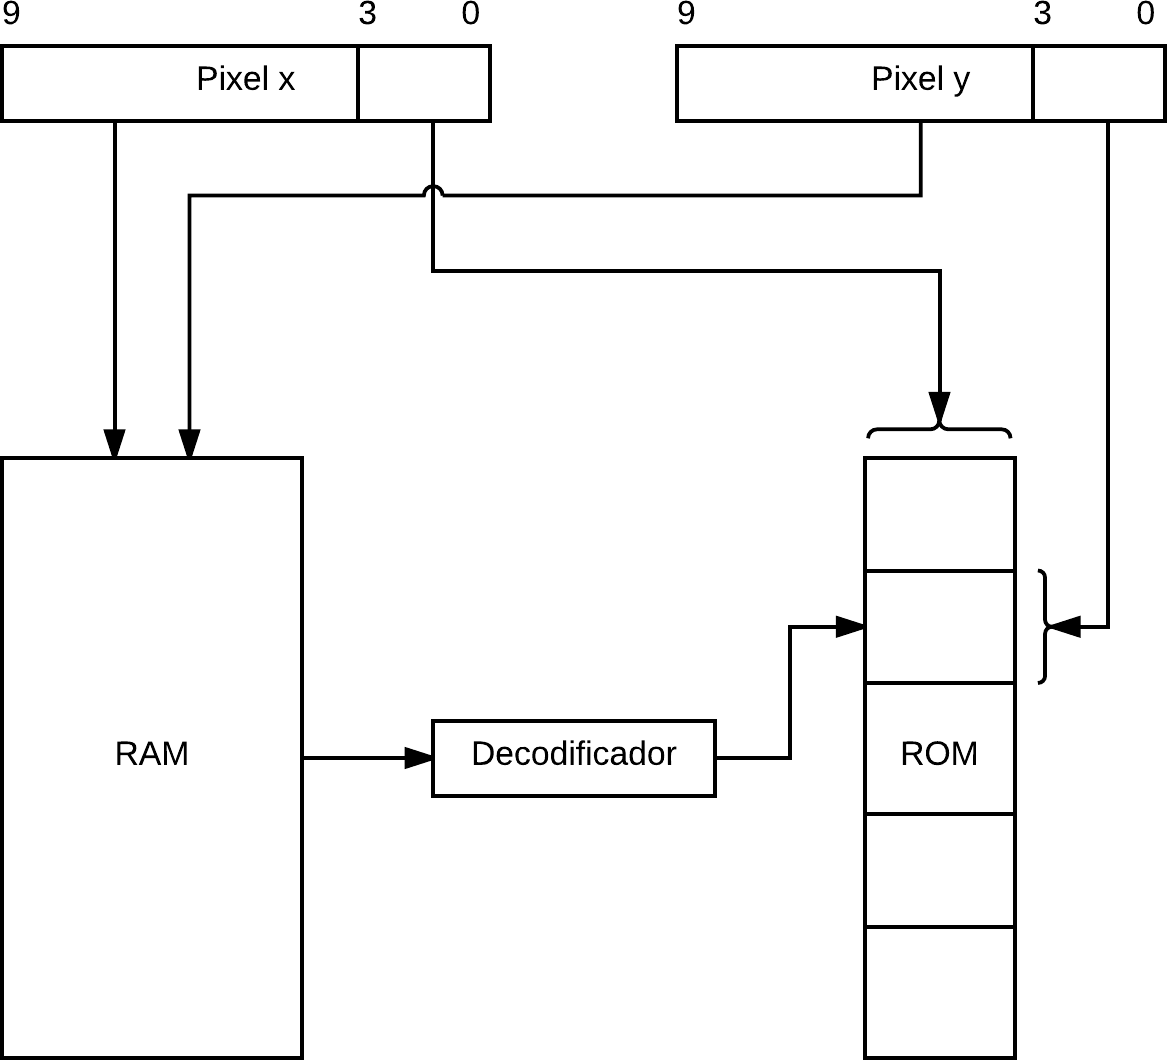
\includegraphics[scale=1]{img/bits.png}
	\vspace{3mm}
	\caption{Endereçamento de dados na RAM e ROM}
	\label{fig:bits}
\end{figure}

O módulo inteiro, desde o seu canal exclusivo de acesso à RAM até o envio
do pixel para o monitor, trabalha a uma frequência de 25.2 MHz, garantida por
um PLL interno. Porém, tanto a RAM quanto a ROM necessitam de pelo menos 1 
ciclo para que o endereço seja enviado para os registradores internos da 
memória e o resultado apareça na saída, para contornar esse problema o
módulo implementa um pequeno \emph{Pipeline} onde os dados decodificados da RAM
são enviados para ROM no mesmo ciclo que um novo endereço é requisitado à RAM.

\begin{figure}[ht!]
	\centering
	\vspace{5mm}
	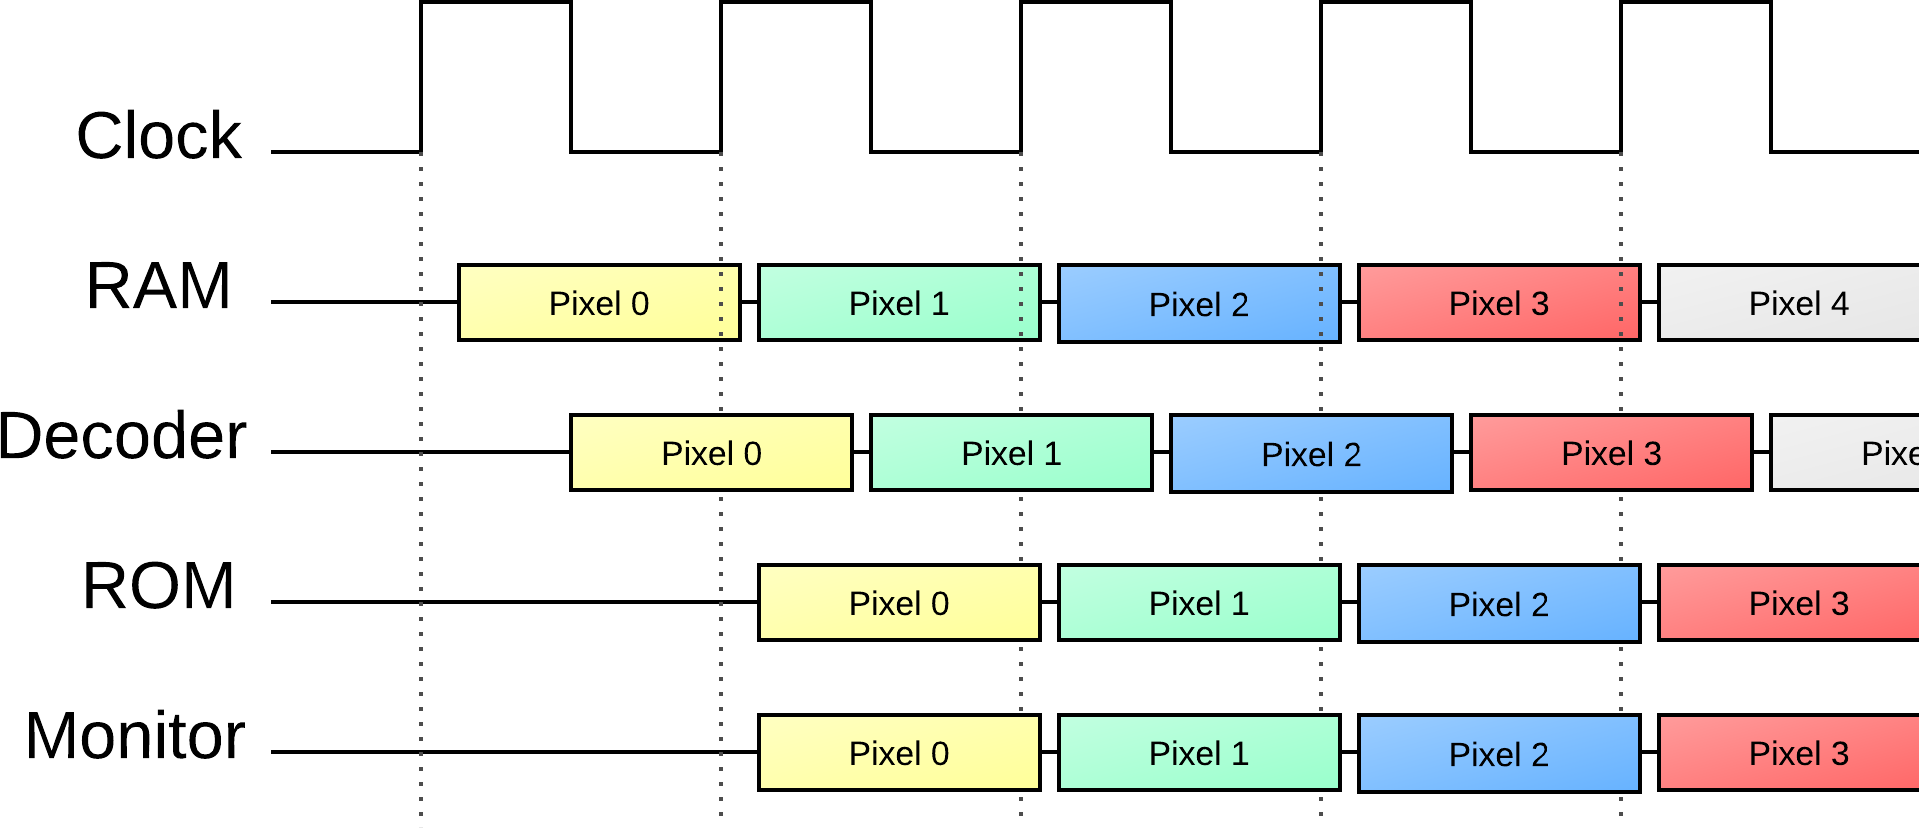
\includegraphics[scale=1]{img/sequence.png}
	\vspace{3mm}
	\caption{Sequência de acesso às memórias feito pela VGA}
	\label{fig:sequence}
\end{figure}

Como visto na figura~\ref{fig:sequence}, a cada ciclo o contador que representa
o pixel na tela é incrementado, então o módulo trabalha com a ideia de 
contadores atrasados. Em um instante $t$ a posição do pixel é utilizada para 
indexar a RAM, no próximo ciclo essa mesma posição estará guardada em um 
registrador (agora representando $t - 1$) e será usada para indexar a ROM 
juntamente com o valor da RAM, no terceiro e último ciclo o contador $t - 2$ indica
efetivamente o pixel que será enviado para o monitor, esse pixel é então 
multiplexado com o mouse e enviado, como visto na figura~\ref{fig:vgacom}.

\begin{figure}[ht!]
	\centering
	\vspace{5mm}
	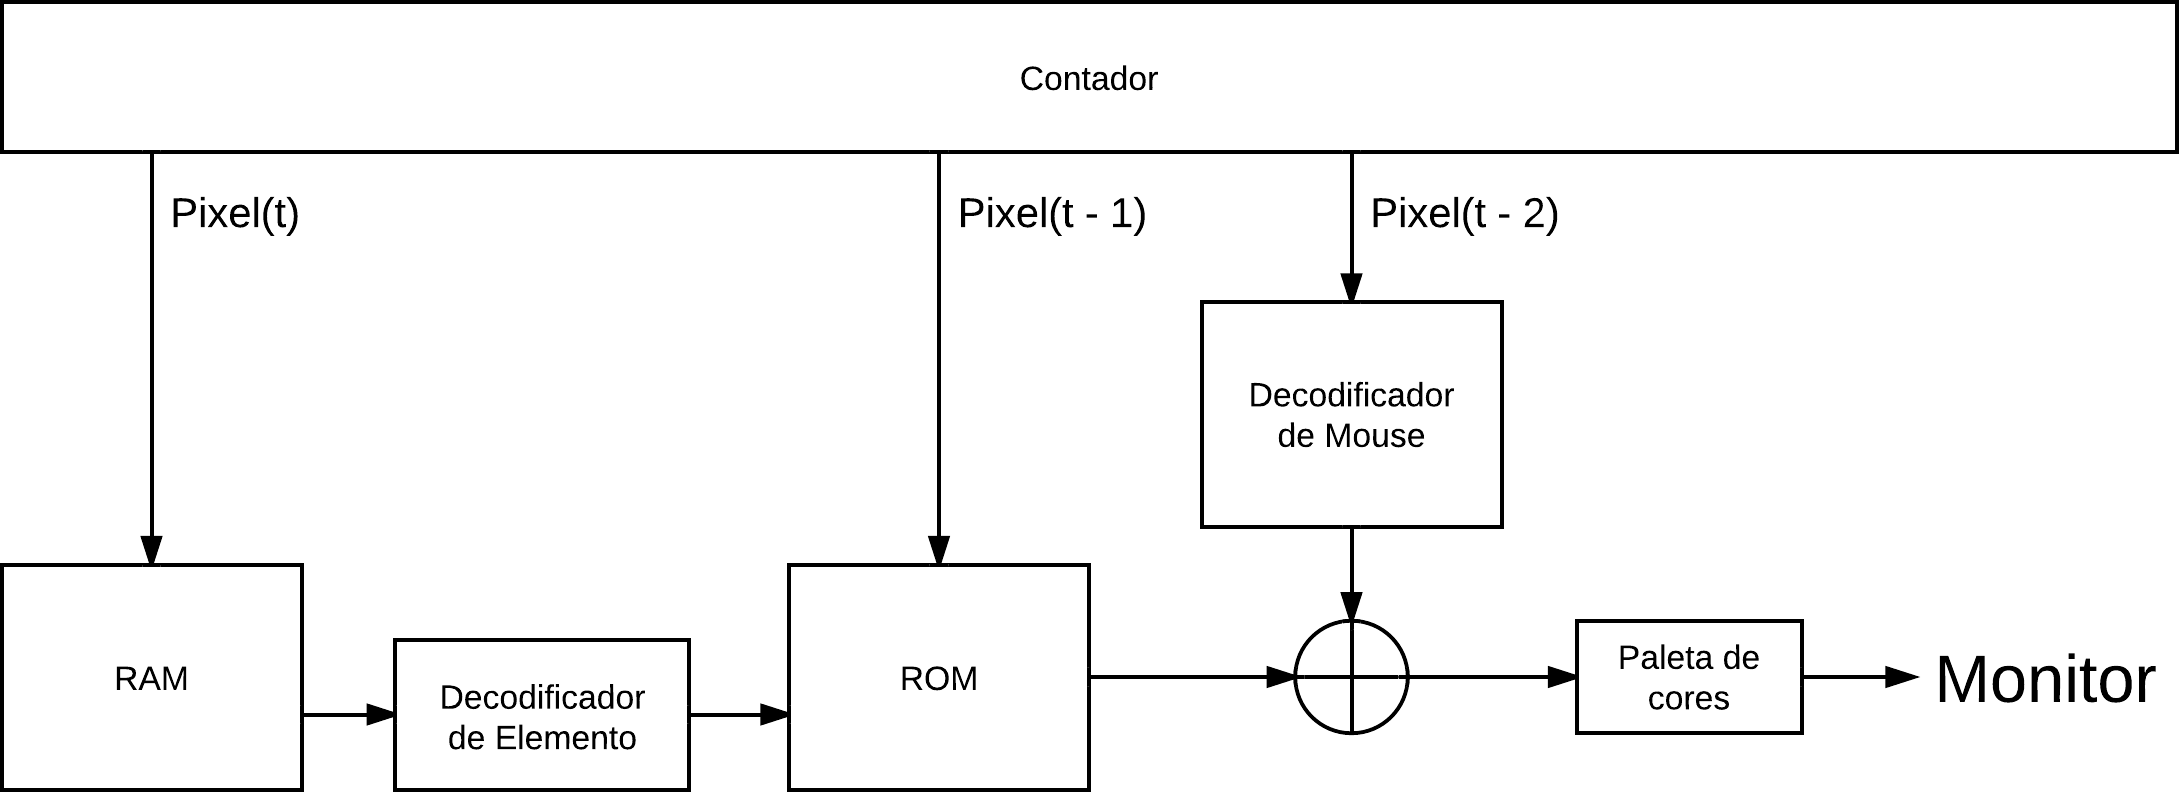
\includegraphics[scale=0.85]{img/components.png}
	\vspace{3mm}
	\caption{Estrutura básica da VGA}
	\label{fig:vgacom}
\end{figure}

A ROM gráfica possui exatamente 16384 palavras de 4 bits, representando uma
entrada na paleta de 16 cores que gera a cor enviada para o monitor. Ela está
organizada de forma a diminuir a lógica combinacional necessária para acessar
cada ladrilho:

\begin{enumerate}

	\item O endereço dos diferentes rostos é obtido diretamente a partir do 
		estado do jogo e do estado do mouse.
		
	\item O endereço dos números é obtido apenas concatenando seus bits em
		BCD aos bits de endereço
		
	\item Campos com números ou vazios, quando abertos, são endereçados de 
		forma similar aos elementos numéricos. Uma lógica combinacional mais elaborada é
		utilizada para validar todas as combinações possíveis de exibição dos
		campos, as expressões de cada possível ladrinho foram montadas em
		função dos \emph{max-termos} e a expressão foi minimizada, um padrão
		xadrez preto e magenta foi utilizado para estados incoerentes (por
		exemplo ter um jogo ganho onde existem campos fechados que não são 
		bombas), facilitando a detecção de erros.

	\item Elementos estruturais tem seu endereço salvo integralmente na RAM,
		seu endereço na ROM se reduz a uma simples atribuição de bits.

\end{enumerate}

Cada um dos 4 decodificadores (um para cada classe de elemento) foi 
implementada em um módulo separado e seus resultados foram multiplexados pelo
tipo de elemento (2 bits mais significativos), isso garantiu uma boa 
modularidade na hora de implementar e corrigir erros.

% Controlador de Mouse %%%%%%%%%%%%%%%%%%%%%%%%%%%%%%%%%%%%%%%%%%%%%%%%%%%%%%%%

\subsection{Controlador de mouse}
\label{sec:ctrlmouse}

{\bf Módulo principal:} \verb|ps2_mouse.vhd|

{\bf Descrição:} O controlador de mouse foi pouco modificado da versão 
fornecida originalmente, ele foi adaptado para permitir posições que variam de
0 a 640 em $x$ e 0 a 480 em $y$. Para isso foi utilizado um conjunto a mais de
variáveis no processo para guardar as posições estritamente dentro da faixa
desejada enquanto as variáveis originais poderiam ser alteradas sem provocar
instabilidade na posição final.

% Unidade de Controle %%%%%%%%%%%%%%%%%%%%%%%%%%%%%%%%%%%%%%%%%%%%%%%%%%%%%%%%%

\subsection{Unidade de controle}
\label{sec:ctrlu}

{\bf Módulo principal:} \verb|game_ctrlunit.vhd|

{\bf Descrição:} Ao invés de separarmos as lógicas de inicialização, jogo e 
pilha em módulos que
precisariam ser sincronizados, optamos por condensar todos os estados em apenas
uma unidade principal de controle. A unidade de controle do jogo se encarrega 
de todos os estados desde o \emph{reset} até o término do jogo. A figura
~\ref{fig:states} mostra os 3 principais grupos da unidade de controle, 
juntamente com os estados inicial e final.

\begin{figure}[ht!]
	\centering
	\vspace{5mm}
	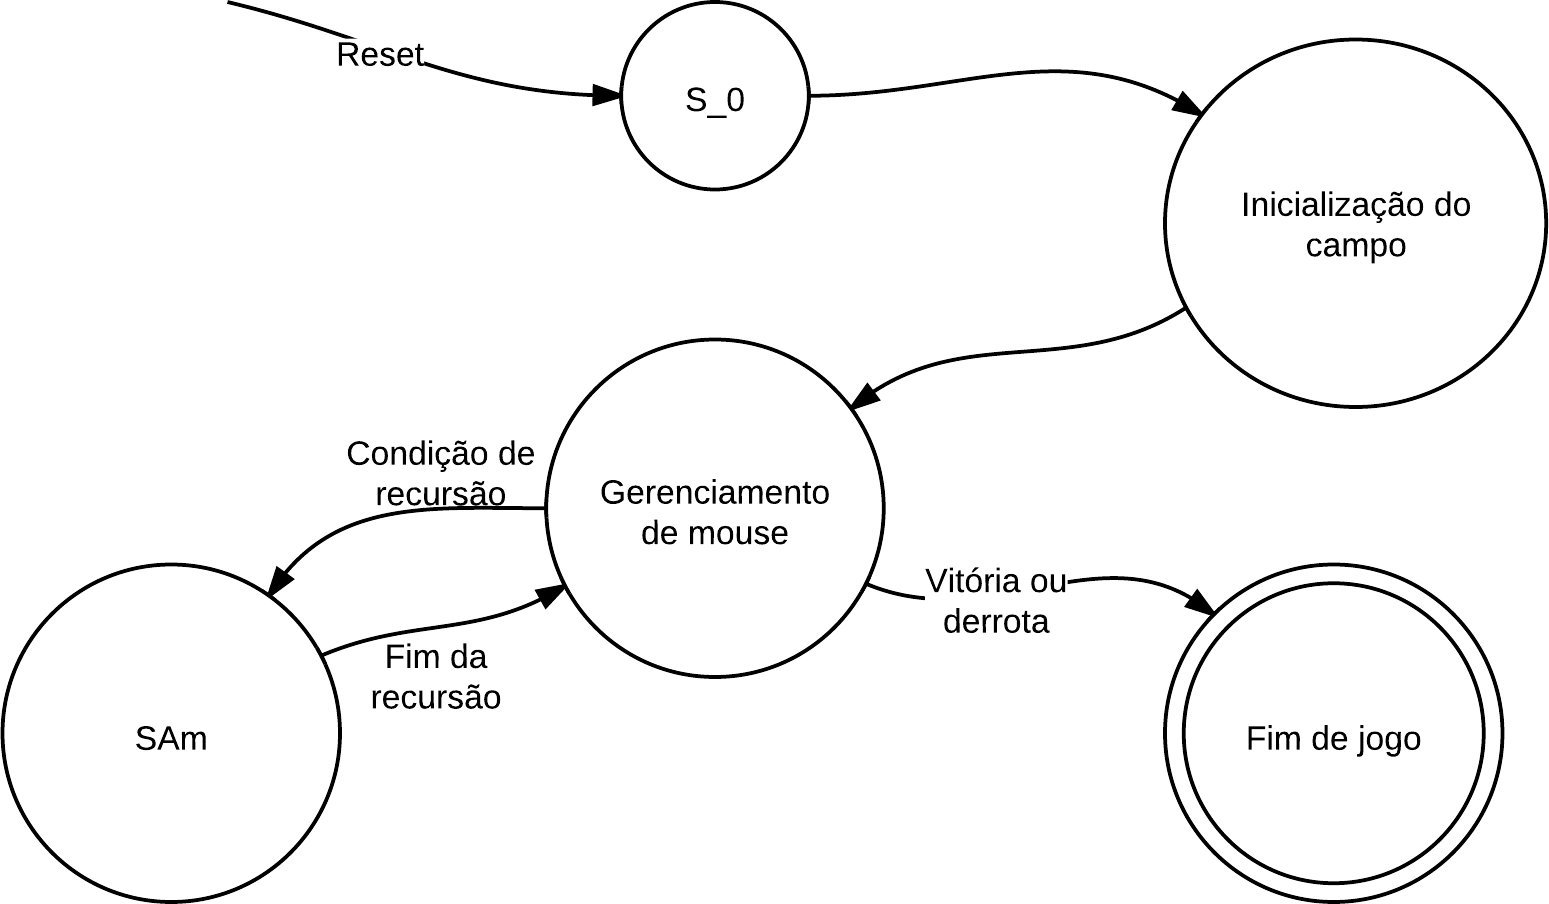
\includegraphics[scale=1]{img/estados.png}
	\vspace{3mm}
	\caption{Diagrama de grupos de estados}
	\label{fig:states}
\end{figure}

% Inicializacao %%%%%%%%%%%%%%%%%%%%%%%%%%%%%%%%%%%%%%%%%%%%%%%%%%%%%%%%%%%%%%%

\subsubsection{Inicialização}
\label{sec:init}

A inicialização possui o maior conjunto de estados da unidade de controle, ela
limpa o campo, inicializa com o número escolhido de minas, evitando repetição
e inicializa os vizinhos das minas com o número de minas visíveis correto.

A lógica responsável pela inicialização dos vizinhos trabalha em conjunto com a
colocação das minas ao invés de analisar todo o campo após a colocação de minas
estar concluída. Quando uma mina é colocada a unidade de controle incrementa
o contador de minas de seus 8 vizinhos se eles forem elementos de jogo e não 
forem minas, o estado responsável utiliza um contador para calcular o endereço
de cada vizinho.

\begin{enumerate}

\item \verb|S_IClr|: Estado responsável por pré-inicializar todos os campos do
	jogo como fechados, não minas, sem bandeiras e com zero vizinhos minas. 
	Após concluir a pré-inicialização ele transita para \verb|S_IRng|.
	
\item \verb|S_IRng|: Obtém um valor aleatório do módulo RNG, verifica se a
	posição faz parte do campo, ele permanece no estado até obter um par
	linha-coluna válido. Quando o par é válido, carrega ele no registrador de
	endereço da RAM e transita para \verb|S_IRdM|.
	
\item \verb|S_IRdM|: Envia o endereço para os registradores internos da RAM e
	aguarda. Transita para \verb|S_IChkM|.
	
\item \verb|S_IChkM|: Verifica se o campo já é uma mina, se for volta para o 
	estado \verb|S_IRng|, se não for habilita a escrita com o padrão de bits
	de uma mina, zera o contador que será usado para preencher os vizinhos e
	transita para \verb|S_IWrM|.
	
\item \verb|S_IWrM|: Espera os dados serem enviados para os registradores da
	RAM. Transita para \verb|S_IChkN|.
	
\item \verb|S_IChkN|: Calcula o endereço do vizinho baseado em um contador.
	Transita para \verb|S_IRdN|.
	
\item \verb|S_IRdN|: Carrega o endereço para a RAM e espera a memória.
	Transita para \verb|S_IIncN|.
	
\item \verb|S_IIncN|: Verifica se o vizinho é um elemento de jogo e não é
	uma mina, carrega o valor incrementado do contador de minas para a 
	memória e habilita a escrita da RAM. Transita para \verb|S_IWrN|.
	
\item \verb|S_IWrN|: Aguarda a escrita do novo contador de minas para a 
	RAM. Transita para \verb|S_IRng| se o contador de vizinhos estourar, 
	se não volta para \verb|S_IChkN|.

\end{enumerate}

% Mouse %%%%%%%%%%%%%%%%%%%%%%%%%%%%%%%%%%%%%%%%%%%%%%%%%%%%%%%%%%%%%%%%%%%%%%%

\subsubsection{Mouse}
\label{sec:mouse}

Como o jogo depende explicitamente de uma ação de clique do mouse, o grupo de
estados que controlam o mouse, mais especificamente o que aguarda uma ação, são
o ponto de retorno de todos os grupos estados. Outra função desse grupo é
garantir que as ações só sejam executadas quando o jogador solta um dos botões,
isso é importante pois é o momento em que percebemos que erramos algo, 
possibilitando que o jogador escolha outro campo antes soltar o botão.

\begin{enumerate}

\item \verb|S_MW|: Aguarda um clique do mouse, de algum dos 2 botões, o valor é
	guardado em registradores durante a subida do \emph{clock} pois mantém o 
	valor dos botões estável. Carrega para o registrador de endereço da RAM a
	posição atual do mouse para já ter o valor do campo sob o mouse disponível
	quando for modificá-lo. Transita para \verb|S_MHL| ao pressionar o botão
	esquerdo e \verb|S_MHR| ao pressionar o botão direito. Por ser o estado
	principal do jogo ele verifica a condição de vitória, nesse caso, transita
	para o fim de jogo e alterando o estado para ganho.
	
\item \verb|S_MHR|: Aguarda o botão direito ser solto e continua carregando a
	posição do mouse para o registrador de endereço da RAM. 
	Transita para \verb|S_MR|.
	
\item \verb|S_MHL|: Aguarda o botão esquerdo ser solto e continua carregando a
	posição do mouse para o registrador de endereço da RAM. 
	Transita para \verb|S_ML|.
	
\item \verb|S_MR|: Tenta colocar/tirar uma bandeira no campo sob o mouse, testa
	se o campo é um elemento do jogo e ainda não foi aberto, habilita a escrita
	da RAM onde os bits de entrada são idênticos os de saída, exceto com o bit 
	F invertido. Decrementa/Incrementa o contador de minas e transita para 
	\verb|S_MW|.
	
\item \verb|S_ML|: Garante que a informação tenha sido trazida da RAM.
	Transita para \verb|S_MOpen|.

\item \verb|S_MOpen|: Tenta abrir o campo sob o mouse, verifica se o campo 
	é um elemento do jogo, ainda não foi aberto nem possui uma bandeira. Assim
	como na colocação da bandeira, o novo valor para a RAM é o mesmo, mas dessa
	vez invertendo o bit C. A condição de abrir o campo também inicia o 
	contador de tempo do jogo. Caso o campo seja uma mina ele altera o estado
	do jogo para derrota e transita para o fim do jogo, se não, além de abrir
	ele também decrementa o contador de campos abertos. Ocorre também a
	verificação de recursão, caso o campo seja um campo vazio (que não enxerga
	minas nos seus vizinhos) ele habilita uma operação de \emph{push} na pilha
	com o endereço atual do campo e um contador zero nos bits mais 
	significativos. O estado transita de volta para \verb|S_MW| caso não haja
	recursão, se não ele transita para \verb|S_SAmPush|, o ponto de entrada do
	SAm.
	
\end{enumerate}

% SAm %%%%%%%%%%%%%%%%%%%%%%%%%%%%%%%%%%%%%%%%%%%%%%%%%%%%%%%%%%%%%%%%%%%%%%%%%

\subsubsection{\underline{S}tack \underline{A}uto\underline{m}ata (SAm)}
\label{sec:sam}

SAm é o conjunto de estados responsável por desenrolar a recursão criada por
causa de campos vazios: Quando um campo é vazio ele abre todos os campos a sua
volta, portanto vizinhos vazios também deverão abrir os campos a sua volta. O
SAm utiliza uma pilha implementada em \emph{hardware} para permitir que o
processo de abertura de um campo possa ser interrompido para seu vizinho
começar o mesmo processo. A recursão se inicia partindo o princípio que a
pilha contém um elemento inicial e termina quando a pilha esvazia. O SAm é
compacto em número de estados principalmente porque a pilha é implementada
separada da RAM, permitindo que operações possam ser feitas em paralelo nas
duas.

\begin{enumerate}

\item \verb|S_SAmPush|: Aguarda a operação ser processada pela pilha. Transita
	para \verb|S_SAmProc|.
	
\item \verb|S_SAmProc|: Verifica a base da recursão, se a pilha estiver vazia
	transita para \verb|S_MW|. Se a pilha não estiver vazia calcula o endereço
	do próximo vizinho baseado no endereço e contador salvos na pilha, se o
	contador for 7 (o último possível vizinho) então uma operação de \emph{pop}
	é enviada para a pilha, caso contrário uma operação de \emph{overwrite}
	atualiza o contador com o valor incrementado, mantendo o endereço. Quando a
	recursão tem continuidade, o próximo estado é o \verb|S_SAmUpdate|.
	
\item \verb|S_SAmUpdate|: Aguarda tanto a pilha quanto o carregamento do 
	elemento vizinho na RAM. Transita para \verb|S_SAmOpen|.
	
\item \verb|S_SAmOpen|: O último estado do SAm valida o elemento vizinho,
	verificando se ele é válido para ser aberto (é um elemento do jogo, não
	possui bandeira nem já foi aberto), abre-o e verifica também se ele é um
	candidato a continuar a recursão (elemento vazio), se for candidato uma
	operação de \emph{push} é enviada com o endereço desse vizinho e um
	contador zerado nos bits mais significativos. O estado também decrementa o
	contador de campos abertos e transita de volta para o \verb|S_SAmPush| para 
	atualizar a pilha e a memória.

\end{enumerate}

% Outros %%%%%%%%%%%%%%%%%%%%%%%%%%%%%%%%%%%%%%%%%%%%%%%%%%%%%%%%%%%%%%%%%%%%%%

\subsection{Outros componentes}
\label{sec:others}

Para o projeto fizemos uso de vários componentes auxiliares como os 
decodificadores BCD usados em laboratórios, contadores para o contador de
tempo, um divisor de \emph{clock} baseado também em um laboratório e um 
decodificador de binário para BCD de 3 dígitos, que utiliza divisão é modulo.

% Conclusao %%%%%%%%%%%%%%%%%%%%%%%%%%%%%%%%%%%%%%%%%%%%%%%%%%%%%%%%%%%%%%%%%%%

\section{Conclusão}
\label{sec:conclusion}

Esse projeto foi interessante por combinar conceitos não apenas de circuitos
lógicos (SAm) e por nos fazer lidar com diversos estados e garantir que a
informação permanecesse coerente durante cada transição bem como a necessidade
de saber exatamente o que cada módulo está fazendo enquanto a máquina de 
estados está trabalhando. Encontramos problemas principalmente para garantir
que os estados que lidam com o mouse não travassem por causa de cliques rápidos
ou oscilações e para garantir que uma estrutura na RAM que fosse fácil o 
suficiente para entendermos e trabalharmos tanto do lado da unidade de controle
quanto da VGA. Apesar dos diversos avisos do Quartus nós estouramos o tempo de
propagação do estado do jogo entre a unidade de controle e a VGA, o que seria
um problema sério se a VGA não fosse praticamente assíncrona em relação à
unidade de control,e com uma taxa de atualização suficientemente rápida.
Apesar de algum comandos não terem sido implementados, como o clique com o 
botão esquerdo e direito ao mesmo tempo, todas as especificações iniciais do
projeto foram implementadas.

% FIM %%%%%%%%%%%%%%%%%%%%%%%%%%%%%%%%%%%%%%%%%%%%%%%%%%%%%%%%%%%%%%%%%%%%%%%%%
\end{document}